\documentclass[11pt,a4paper]{report}

\usepackage[dvipdfm]{graphicx}
\usepackage[driverfallback=hypertex]{hyperref}
\usepackage{amsmath}
\usepackage{amsfonts}
\usepackage{amssymb}
\usepackage{latexsym}
\usepackage{fancyhdr}
\usepackage{float}
\usepackage{subfig}
\usepackage{bmpsize}


\DeclareMathOperator{\power}{\mathcal{P}}

\begin{document}

\title{Understanding how to attack DES via SAT}
\author{David William Jones - 635773}

\maketitle
\tableofcontents

\chapter{Introduction}
\label{cha:Introduction}

\section{Motivation}
\label{cha:Motivation}

Encrypting messages and decrypting messages has held an interest with me along with the secrecy surrounded by cryptology. The main thing that fascinates me about encryption is that pieces of text can be transformed into illegible messages and then back again with the use of a key. This project will be an accomplishment if i can outline existing documentation to build a theoretical framework to translate DES to SAT. This will make it easier to understand the concepts needed to break DES. Once I have this framework of knowledge, it will be able to guide me through the process of breaking DES with the use of experiments. I hope this will be useful to other researchers in closely related fields as they will be able to use some of the methods, explanations for their work or help explain to students DES and its link with SAT.



\section{Aims of the project}
\label{cha:Aims}

The project will be focused on constructing an understanding of the Data Encryption Standard (DES), where one is able to encrypt messages and decrypt a message via a key. The second part of the project is to study SAT to gain an understanding of the subject so it can then start to be linked into the attacking of DES. Additionally the DES should be applied and developed into a Conjunctive Normal Form.
The aims of the project should be left open throughout the different stages of the project as this is a theoretical paper. Discoveries through the paper may open up other areas of interest that one could look deeper into these topics that arise.

The aims of the project:

\begin{enumerate}
\item Research and study the Data Encryption Standard.
\item Understanding the fundamental basics of Satisfiability and Boolean functions.
\item Understanding and document the existing translation of DES to SAT.
\item To develop a Data Encryption Standard via Conjunctive Normal Form.
\item Test the CNF's in a SAT solver and find methods to improve aspects of the computation.
\item Show the improvement of the existing facilities with the use of experiments.
\end{enumerate}


\section{Science engineering}
\label{sec:sciEng}
The main aim of the project has already been declared, but there are additional objectives which must be taken into account when writing the research paper.
\begin{enumerate}
\item Learn and use the software \LaTeX \space to write the dissertation.
\item Install and understand how to use Git and Github, to keep track of the progress of the project with the supervisor.
\end{enumerate}
\LaTeX \space is a writing environment which gives the user more control when constructing a paper over more popular software such as Microsoft Word. A detailed analysis of the advantages of using such a software can be found in \ref{sec:LaTeX}.
Github is a file sharing hosting service which allows one or more person to work on a project on their own machines. A detailed description of Github can be found in \ref{sec:Git}



\section{Related Work}
\label{cha:RWork}

There have been some published papers which are similar to the topic area, but not many. A basic understanding and framework can be taken from these papers to develop a well designed structure to the projects work.

The interaction between Propositional Satisfiability and Applications in Cryptography and Ramsey Problems \cite{Gwynne2010Interaction} is a recently published thesis that looks at a different encryption standard called Advanced Encryption Standard (AES). The paper first of all outlines and declares what Boolean functions are and SAT. The thesis paper goes into depth of how the AES works by giving a very detailed explanation along with examples of how it is runs. Then there is a translation of AES into SAT with the use of Conjunctive Normal Form (CNF). The framework within the thesis provided a translation of satisfiability theorems to be used in encryption. A lot of the work talks about breaking AES which is a successor of DES. However techniques used to break AES can be adopted and will be closely linked to DES.
Other work such as Logical Cryptanalysis as a SAT Problem \cite{Fabio2000LogicalSAT} outlines DES which gives a great framework to use, covering everything step by step from the initial permutation to the generation of keys.

There are other cryptanalysis techniques which include differential cryptanalysis. Differential cryptanalysis was the first method to break DES faster than the previous brute force method that the exhaustive search did. The method is based up having a device which can encrypt data with a hard-wired secret key, and we assume that we don't have the tools to `read' the key within a chip. What we then do, is to choose some blocks of data and to encrypt them with the device. The data analysis will then compute the key by analysing roughly $2^{47}$ chosen plain text bits \cite{Junod2013LASEC}. This reduced  the probability of success as we cut out a lot of computation compared to 2$^{56}$.




\chapter{Analytical Background}
\label{cha:AnBack}

The analytical background will first describe the terminology used throughout this paper. This gives students that are new to the area of cryptology an understanding of what some of the words are defined as.


\section{Terminology}
\label{sec:Term}
A description of the definitions to impose a level of abstraction.

\paragraph{Cryptography}
The study of encryption and decryption to keeping secrets a secret \cite{DBLP:series/isc/DelfsK07}.

\paragraph{Cryptography}
The study of encryption and decryption to keeping secrets a secret \cite{DBLP:series/isc/DelfsK07}.

\paragraph{Encryption}
The process of transforming a sequence of bits into another sequence of bits with certain properties \cite{Fabio2000LogicalSAT}.

\paragraph{Decryption}
The process of mapping back the cipher text into the plain text with the use of a key \cite{Fabio2000LogicalSAT}.

\paragraph{Cryptanalysis}
The science of studying attacks against cryptographic schemes. Successful attacks may, for example, recover plain text (or parts of the plain text) from the cipher text \cite{DBLP:books/sp/Buchmann02}.

\paragraph{Plain text}
A message that holds meaning to the user that is to be transmitted \cite{DBLP:books/sp/Buchmann02}.

\paragraph{Cipher text}
The result of encryption performed on a plain text using an algorithm \cite{Berti2003CISSP}.

\paragraph{Key}
A Key is used to encrypt and decrypt a message \cite{Berti2003CISSP}.

\paragraph{Boolean functions}
A logical operation were each operands will take the result of one of two values \cite{Gregory2013Cryptanalysis}.

\paragraph{Intervertebral function}
An intervertebral function allows you to carry out the
same process from getting state 1 to state 2. As a result the same process
allows us to get from state 2 to state 1.

\paragraph{Permutation}
Given D is a set, a \emph{permutation} of D is a bijective mapping of
\begin{displaymath}
F: D \rightarrow D
\end{displaymath}
with the original values being in the output but rearranged. In other words, what is represented in the input of D will be found in the output of D.

An example of a permutation would be is that there is a total of 6 permutations available for the set \{a,b,c\} which are:
\begin{center}
(a,b,c) (a,c,b) (b,a,c) (b,c,a) (c,a,b) (c,b,a).
\end{center}


We use the following \textbf{formal notation}:
\begin{description}
\item[M] Message
\item[P] Plain text
\end{description}
C = Cipher text
K = Key
E = Encryption algorithm
D = Decryption algorithm
E$_{K}$ = Encryption Key
D$_{K}$ = Decryption Key

\section{General Cryptography}
\label{sec:GenCrypt}
Cryptography is the study of encryption and decryption to keep data a secret \cite{DBLP:series/isc/DelfsK07}. It has been around for centuries with one of the first examples being the “Caesar cipher” which was used around 40BC. This is probably one of the more famous examples of encryption.
Encryption is important because people have secrets and want to keep the information they are transmitting hidden from people who would manage to intercept the message. If we say for example “Bob” wants to send a message “x” to “Alice”. If this message is sent to Alice without any encryption and it is intercepted by say “Eve”, then "Eve" is able to read said message “x”, thus no longer making “x” a secret. However encryption can help keep “Bobs” message a secret from “Eve”. This is done by at the most basic level, applying an encryption method to the message to produce a cipher text. The cipher text can then be passed on to “Alice”. If the message “x” is intercepted by “Eve”, then the message will be incoherent to read. This is because the encryption will have changed the message on the Plain text into something new which no longer resembles the original message. Once “Alice” has the cipher text, she can now apply a decryption method to the cipher text to read the original message. It is important to note that “Alice” is able to decrypt the cipher text by using a key that both parties will have agreed on before the transmission of a message “x”. This in essence is how encryption and decryption is used.

\textbf{Encryption notation}
\begin{displaymath}
C = E (K, P)
\end{displaymath}
The notation for encryption shows that putting the Key and the Plain text into the encryption algorithm will output a Cipher text.

\textbf{Decryption notation}
\begin{displaymath}
P = D (K, C)
\end{displaymath}
The notation for decrypting shows that putting the Cipher text and key together in the decryption algorithm will output a Cipher text.

\textbf{Symmetric and asymmetric encryption}
Symmetric-key encryption schemes provide secure communication for a pair of communication partners \cite{DBLP:series/isc/DelfsK07}. Symmetric-key encryption algorithms have the fastest implementations in hardware and software. Therefore, they are very well-suited to the encryption of large amounts of data \cite{DBLP:series/isc/DelfsK07}. In symmetric encryption the encryption key will always be the same as the decryption key. We there for say within asymmetric encryption that E$_{K}$ = D$_{K}$. This is seen and proven in the encryption and decryption notation as both P and C can be interchanged to produce either the Plain text or Cipher text respectively.In asymmetric encryption the encryption key and decryption key are unique and the computation of decryption from encryption is infeasible. Compared to symmetric encryption, the asymmetric encryption key can be made public \cite{DBLP:series/isc/DelfsK07}. However the decryption key is still kept a secret. Because anyone can use the encryption key it is called the “public” key. For a public key it is useful to have two different key spaces since the public key and the private key are shaped differently \cite{DBLP:series/isc/DelfsK07}.

\textbf{RSA}
RSA is named after its inventors Ron Rivest, Adi Shamir and Len Adleman. RSA was the first public-key cryptosystem and is still one of the most important \cite{DBLP:series/isc/DelfsK07}. The most important thing to note about RSA is that it is an asymmetric encryption method and so therefore has a public key and a private key. Both keys however are mathematically linked. The public key is known to everyone and is used to decrypt messages. On the other hand the private key is used to encrypt messages. The general idea behind the encryption of RSA is that the factors of the two generated messages cannot be recovered from $n$. RSA will generate two different random numbers which are odd prime numbers. The product is then taken from these values. A new value (e) is then introduced which is a prime number relative to $n$. The pair (n, e) is then the public key. The decryption is then computed with ne $\equiv$ 1 mod (n). (n,d) is then used as the private key. This is just one of the other possible methods of encryption available.


\section{Sets}
\label{sec:sets}

A set is a collection of objects. To show that an object $x$ is in the set $X$ we use the membership symbol ($\in$) to show that $x$ belongs in something. This will be written as $x \in X$. Sets can be elements of other sets which are referred to as subsets. To show that all subsets of a set $X$ we write it as $\power(X)$. Two sets are equivalent if they have the same exact elements in both of the sets. It should be noted that although the two sets have the same elements, the sets themselves can mean different things. Set $X$ is in set $Y$ if all elements of $X$ are an element of $Y$.
Therefore we can say for the sets $X$ and $Y$:
\begin{center}
  $X=Y$ if and only if $X \subseteq Y$ and $Y \subseteq X$.
\end{center}
A set can have nothing within inside it (no elements) which is referred as the empty set. The empty set is denoted as the symbol $\emptyset$ or $\{\}$. There are four operations that can be applied to sets that can produce new sets.

\subsection{The four basic operations}
\label{sec:fourbasop}

The \emph{intersection} operation takes two sets and finds the element that occur in both set $X$ and set $Y$, $X \cap Y$. Therefore intersection is:
\begin{displaymath}
  X \cap Y = \{x : x \in X  \text{ and } x \in Y\}.
\end{displaymath}

The \emph{union} operation takes two sets to find an element that is in either both of the two sets or belongs in the set $X$ or $Y$, $X \cup Y$. Therefore the union of sets $X$ and $Y$ is:
\begin{displaymath}
  X \cup Y = \{x : x \in X  \text{ or } x \in Y\}.
\end{displaymath}

The \emph{difference} operation finds an element that is in set $X$ but not in set $Y$, $X \setminus Y$. Therefore the difference of sets $X$ and $Y$ is:
\begin{displaymath}
  X \setminus Y = \{x : x \in X  \text{ and } x \notin Y\}.
\end{displaymath}

The sets we have been talking about up to this point have elements within them that are not dependant on the order they are in. For example the set $\{x,y\}$ is the same as the set $\{y, x\}$ as they both have the same elements. However we can have ordered sets were the position of a element within the set is important and makes the set unique. To define a set that is ordered we use parentheses  ``$()$'' , i.e., $(x,y)$.
The (Cartesian) product of sets $X, Y$ is
\begin{displaymath}
  X \times Y = \{(x,y) : x \in X \text{ and } y \in Y\}.
\end{displaymath}
A \emph{relation} is a subset of the product of sets, which is written as $R \subseteq X \times Y$. A \emph{function} (or \emph{map}) relates an input to an output. Functions are denoted by a small ``$f$'' followed by its input. A simple example of this would be $f(x) = x^2$. Using the variable x for when $x=4$ the function will therefore be, $f(x) = 16$.




\chapter{Block Ciphers}
\label{cha:BCipher}

A block cipher is defined as a symmetric-key encryption scheme with
\begin{displaymath}
 M = C = \{0,1\}^{n}
\end{displaymath}
 $n$ is the block length of the cipher \cite{DBLP:series/isc/DelfsK07}. Block ciphers are used to encrypt blocks of bits of a fixed length to a new different output \cite{DBLP:books/sp/Buchmann02}. For example if the input length of a block cipher is 8 bits, then the output block cipher will also be 8 bits long. A block cipher is referred to as a cryptosystem if its plain text and cipher text are of the same length.A block cipher will map an original Plain text into a cipher text with the use of permutation. Block ciphers are closely related to binary arithmetic in how to calculate the new values and current values of which will be shown later.
A block cipher is made up of two algorithms which we will call E and D (Encryption and decryption algorithm). Both of these algorithms take in a key called K. Given a Plain text (PT) the encryption will take in a key and map both these inputs to an output. This output is the Cipher text (CT). This can be seen in Figure \ref*{fig:2.2.1}


\begin{figure}[H]
\centering
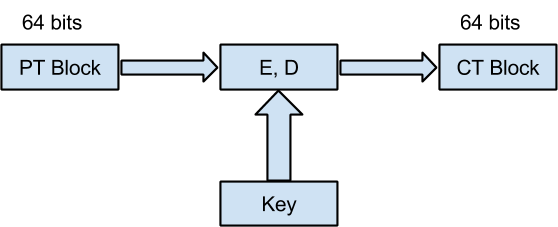
\includegraphics[scale=0.5]{BlockCipher.png}
\caption{Illustration of a block cipher.}
\label{fig:2.2.1}
\end{figure}



The reason block ciphers are useful is that it takes in $n$ inputs and outputs $n$. Block ciphers are built by iteration were they take in as an input a key K. The key K will then be expanded into $K_{1}, K_{2},..., K_{n}$. These are called \emph{round keys}. The cipher will use these round keys by encrypting the message a number of times. So the encryption would work by taking producing a new message with each computation of th message and a key $R: (K_{1}, M)$ respectively. This will produce a message ($m_{1}$) were it will go through the same process with a different key until all the round keys are computed. Once all the rounds are complete one is left with C.

Block ciphers can encrypt messages of arbitrary length. There are different properties and issues that must be looked at regarding the different lengths. First we look at where the plain text is greater than the cipher text (P $\textless$ C). This essentially means that our input is grater than our output. Practically this does not make sense as there will be a lose of data within the cipher text. However an alternative view would be that error checking was in the plain text , so therefore they were parity bits. In this regard this arbitrary block cipher would be acceptable.

An alternative block cipher encryption would be if the plain text contains less bits than the cipher text (P $\textgreater$ C). This will essentially mean that random useless data is added onto the cipher text. As a result of this, in theory, the cipher text is securer in terms of plain text attacking. This is due to the user having to use up more time to try and find meaning to the random useless bits therefore taking more time to crack.

The security of an encryption is determined by its key. Specifically the more key iterations a encryption has, the more secure/ harder it will be to break. A encryption with only one key will encrypt a plain text once. This is less effective in terms of security compared to a plain text that uses more keys. This is due to the fact that the randomness of the cipher text increases.

\emph{Weak keys} in cryptography are keys which when used with a plain text will result in a cipher text with specific properties. These properties are unfavourable as it leads to a security problem. It should be noted that weak keys are rare due to the amount of keys available to encrypt a message, but do raise a major flaw in the security of a message. As a result it is often attempted to reduce the chance of obtaining a weak key. An example of a weak key would be if all the bits are all 1's, 0's or alternating 0's and 1's. The consequence of using a weak key to encrypt a block cipher and then encrypt the result with the same weak key, we will obtain the original block cipher.











There are "basic properties" given with keys to show that keys will always map to different outputs. In other words, if we are given two different keys, there exists a mapping for each key such that there will always be a different output (never both map to the same value). In other words, encryption key 1 (E$_{K1}$) is not equal to encryption key 2 (E$_{K2}$) in terms of mapping to the same cipher text (C).
\begin{displaymath}
E_{K1} \neq E_{K2} \rightarrow C
\end{displaymath}
An example of this would be given a plain text of 1 bit in length that is assigned to binary value 1 and two keys each one bit in length where E$_{K1}$ is assigned to 0 and another key E$_{K2}$ is assigned 1. In the example given below, we are looking for two cipher texts not to be equal.

A toy example of this strong property would be:

\begin{figure}[H]
\centering
\label{tab:assignment of values}
\begin{tabular}{|c|c|c|c|}
\hline
P & E$_{K1}$ & E$_{K2}$ & C \\ \hline
1 & 0 & 1 & {}\\
\hline
\end{tabular}
\caption{Denoting the assignment of values}
\end{figure}
The Cipher text will be the result of using the XOR function (see \ref{Figure:4.2.3}) over the plain text and the E$_{Kn}$ to produce a cipher text C$_n$. The Strong property will hold if both cipher texts are not equal.

\begin{figure}[H]
\centering
\label{tab:XOR function}
\begin{tabular}{|c|c|c|c|c|}
\hline
P & E$_{K1}$ & E$_{K2}$ & P $\oplus$ E$_{K1}$ & P $\oplus$ E$_{K2}$\\ \hline
1 & 0 & 1 & 1 & 0 \\
\hline
\end{tabular}
\caption{XOR function over P and K to produce C.}
\end{figure}

The output of P $\oplus$ E$_{K1}$ is equivalent to saying it is cipher text 1 (C$_1$) and P $\oplus$ E$_{K2}$ is equivalent to cipher text 2 (C$_2$). Therefore we have proven that the output C$_1$ $\neq$ C$_2$.
 As seen in figure \ref{tab:XOR function} two different keys do not map to the same output. As a result this is a "Strong property" of keys which is desirable when looking at the security of a block cipher.

 A \emph{Duplicate key} is a key with the same identical property of another key. This property is deriving the same Cipher text. Given two keys and using the domain Plain text \{P\}* which denotes the set of all possible Plain texts, the key will map \{P\}* to the set of all possible Cipher texts \{C\}*.
 \begin{displaymath}
 \{P\}* \rightarrow \{C\}*
 \end{displaymath}
 The duplicate key is of such that has the identical mapping. The same mapping is therefore defined by two given tables that are both naturally ordered, if and only if each row in the first table matches the second and each row in the second table matches the first table.
 An example of a duplicate key would be given C$_{K1}$(P) which denotes the cipher text using the key K$_1$ from the domain P and C$_{K2}$(P) denotes the cipher text using the key K$_2$ from the domain P where domain P in this case is the same for each Cipher text.


\begin{figure}
\begin{table}[H]
\centering
\label{tab:C1}
\begin{tabular}{|c|c|c|}
\hline
P & K$_1$ & C$_{K1}$ \\ \hline
1 & 0 & 1 \\
1 & 0 & 1 \\
0 & 0 & 0 \\
0 & 1 & 1 \\
\hline
\end{tabular}
\caption{Plain text being mapped to a Cipher text using K$_1$}
\end{table}

\begin{table}[H]
\centering
\label{tab:C2}
\begin{tabular}{|c|c|c|}
\hline
P & K$_2$ & C$_{K2}$ \\ \hline
1 & 0 & 1 \\
1 & 0 & 1 \\
0 & 0 & 0 \\
0 & 1 & 1 \\
\hline
\end{tabular}
\caption{Plain text being mapped to a Cipher text using K$_2$}
\end{table}
\end{figure}

By our previous hypothesis, if we take each row from table \ref{tab:C1} and table \ref{tab:C2} then we can evaluate them as equal. Therefore K$_1$ and K$_2$ map the same Plain text to the Cipher text.

\begin{displaymath}
C_{K1}(P) = C_{K2}(P)
\end{displaymath}












\chapter{The Data Encryption Standard}
\label{cha:DES}

The Data Encryption Standard  or DES was developed by the company IBM in 1977 and originally developed from a design by Horst Feistel. DES was specified in [DESON 1997] which was previously the most widely used symmetric-key encryption algorithm. Governments, banks and applications in commerce took the DES as the basis for secure and authentic communication. However today DES is considered no longer secure (in practise). In October 2000 the US secretary of Commerce announced that the nations new encryption standard would be the successor AES. However most successors of DES are still similar, therefore DES is still important in cryptosystems \cite{DBLP:series/isc/DelfsK07} \cite{DBLP:books/sp/Buchmann02}.

\section{Construction of DES}
\label{sec:conDES}
The basic algorithm to construct a DES is to use a block cipher which encrypts blocks of 64 bits (Plain text) into blocks of 64 bits (Cipher text) using a key with 56 bits (the key length is actually 64 bits but 8 of those bits are used for parity checking and is otherwise ignored by the algorithm) \cite{Fabio2000LogicalSAT}.



\textbf{Formula Notation}
\begin{displaymath}
DES: \{0,1\}^{64} \times \{0,1\}^{56} \rightarrow \{0,1\}^{64}
\end{displaymath}
DES is constructed by taking in a 64 bit Plain text, mapping it to an encryption key which is 56 bits long, which will give a 64 bit Cipher text.

\textbf{Feistel Network}
DES uses an algorithm to encrypt data which is called the Feistel network \cite{DBLP:books/sp/Buchmann02}. It works by using permutation, XOR functions (see \ref{Figure:4.2.3}) and round keys in order to encrypt messages. The Feistel network uses arbitrary functions $f_{1},...,f_{d}$ which maps:
\begin{displaymath}
FeistelNetwork: \{0,1\}^n \rightarrow \{0,1\}^n
\end{displaymath}
The aim of the Feistel network is to build up an intervertebral function
\begin{displaymath}
F: \{0,1\}^{2n} \rightarrow \{0,1\}^{2n}
\end{displaymath}
This function will then encrypt the message (P). We start off with two separate inputs which we will call R$_{0}$ and L$_{0}$ made up of both n bits. The total input is 2n - bits. At the first stage the R$_{0}$ will become the L$_{1}$ without any change as seen on the diagram below. However the L inputs is changed. This is done by taking the R$_{0}$ input and feeding it into the arbitrary function f$_{1}$, and the result is then XOR with L$_{0}$. This output will then become R$_{1}$ input. This process is called one round of the Feistel network.
\begin{figure}[h]
\centering
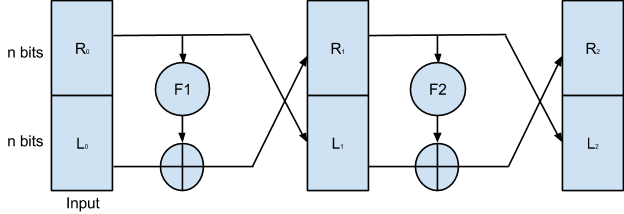
\includegraphics[width=12cm, height=5cm]{FeistelNet.png}
\label{Fig: Feistel Network}
\caption{Illustration of a Feistel Network.}
\end{figure}

This process is carried out until 16 rounds have occurred, which will produce the cipher text. Each round is nearly identical except for the keys, as for each round there is a different subset of 56
key bits that are selected and combined with the input of the previous round \cite{Fabio2000LogicalSAT}.
This can be formulated as (where i = 1,2,...,d):
\begin{displaymath}
L_{i} = R_{i}-1
\end{displaymath}
\begin{displaymath}
R_{i} = F_{i} (R_{i}-1) \oplus L_{i}
\end{displaymath}

The cipher text is then constructed using inverse permutation IP$^{-1}$:
\begin{displaymath}
C = IP^{-1}(R_{16}L_{16})
\end{displaymath}

\subsection{Demonstration of DES}
\label{subsec: DemoDES}

The demonstration will outline how first of all the code is generated and how the input values are determined. If we started with a message, for example:
\begin{displaymath}
M = ABCDEF0123456789
\end{displaymath}
We would rewrite this in a binary format to get our 64 bit plain text. In a table this would look like:

\begin{center}
\begin{tabular}{ |c|c|c|c|c|c|c|c|c| }
\hline
  {} & y$_{1}$ & y$_{2}$ & y$_{3}$ & y$_{4}$ & y$_{5}$ & y$_{6}$ & y$_{7}$ & y$_{8}$ \\ \hline
  x$_{1}$ & 1 & 0 & 1 & 0 & 1 & 0 & 1 & 1 \\ \hline
  x$_{2}$ & 1 & 1 & 0 & 0 & 1 & 1 & 0 & 1 \\ \hline
  x$_{3}$ & 1 & 1 & 1 & 0 & 1 & 1 & 1 & 1 \\ \hline
  x$_{4}$ & 0 & 0 & 0 & 0 & 0 & 0 & 0 & 1 \\ \hline
  x$_{5}$ & 0 & 0 & 1 & 0 & 0 & 0 & 1 & 1 \\ \hline
  x$_{6}$ & 0 & 1 & 0 & 0 & 0 & 1 & 0 & 1 \\ \hline
  x$_{7}$ & 0 & 1 & 1 & 0 & 0 & 1 & 1 & 1 \\ \hline
  x$_{8}$ & 1 & 0 & 0 & 0 & 1 & 0 & 0 & 1 \\ \hline
\end{tabular}
\end{center}

The first 4 cells of each row indicate the binary digit value. As a result the letter A is defined as:

\begin{displaymath}
A \Rightarrow A = \{(x_{1}...x_{1}, y_{1}...y_{4})\}
\end{displaymath}
This translates as A having the binary value `1010', which is the binary for the letter A. Now we have made the connection between Block ciphers and binary arithmetic. The message will then result in a collection of 64 binary digits:

\begin{displaymath}
M = 1010 1011 1100 1101 1110 1111 0000 0001 0010 0011 0101 0110 0111 1000 1001
\end{displaymath}
As we stated before in the Feistel network, we need to split the message into two 36 bit messages. The left and right input will look like:

\begin{displaymath}
Left Input: 1010 1011 1100 1101 1110 1111 0000
\end{displaymath}
\begin{displaymath}
Right Input: 0001 0010 0011 0101 0110 0111 1000 1001
\end{displaymath}
We then want to apply the initial permutation onto our message which maps if:

\begin{displaymath}
p \in \{0,1\}^{64} | p = p_{1}, p_{2}, p_{3}, p_{4},...,p_{64}
\end{displaymath}
As a result, IP must then be:
\begin{displaymath}
IP(_{p}) = p_{47}, p_{23}, p_{52},...,p_{3}
\end{displaymath}

\begin{center}
\begin{tabular}{ |c|c|c|c|c|c|c|c| }
\hline
1 & 1 & 0 & 0 & 1 & 1 & 0 & 0\\ \hline
0 & 0 & 0 & 0 & 0 & 0 & 0 & 0\\ \hline
1 & 1 & 0 & 0 & 1 & 1 & 0 & 0\\ \hline
1 & 1 & 1 & 1 & 1 & 1 & 1 & 1\\ \hline
1 & 1 & 1 & 1 & 0 & 0 & 0 & 0\\ \hline
1 & 0 & 1 & 0 & 1 & 0 & 1 & 0\\ \hline
1 & 1 & 1 & 1 & 0 & 0 & 0 & 0\\ \hline
1 & 0 & 1 & 0 & 1 & 0 & 1 & 0\\ \hline
\end{tabular}
\end{center}
The new mapping of IP gives us Table(a). We can then apply a key to this table to produce our first round table.

\begin{tabular}{|c|c|c|c|c|c|c|c|c|} \hline
K = & 0001 & 0011 & 0011 & 0100 & 0101 & 0111 & 0111 & 1001
\\ \hline
\end{tabular}

\begin{center}
\begin{tabular}{|c|c|c|c|c|c|c|c|} \hline
1001 & 1011 & 1011 & 1100 & 1101 & 1111 & 1111 & 0001\\ \hline
\end{tabular}
\end{center}
We then will compute the XOR as stated by the Feistel network. So as a result the R$_{0}$ will become R$_{1}$ which will be computed on the next round.

This result will be as

\begin{center}
\begin{tabular}{|c|c|c|c|c|c|c|c|} \hline
C$_{0}$ & 1111 & 0000 & 1100 & 1100 & 1010 & 1010 & 1111\\ \hline
D$_{0}$ & 0101 & 0101 & 0110 & 0110 & 0111 & 1000 & 1111\\ \hline
C$_{1}$ & 1110 & 0001 & 1001 & 1001 & 0101 & 0101 & 1111\\ \hline
D$_{1}$ & 1010 & 1010 & 1001 & 1001 & 1110 & 0011 & 1110\\ \hline
\end{tabular}
\end{center}

Using the key one would XOR both C$_{1}$ and D$_{1}$ and will get:

\begin{center}
\begin{tabular}{|c|c|c|c|c|c|c|c|c|c|c|c|c|}\hline
K$_{1}$ & 0001 & 1011 & 0000 & 0010 & 1110 & 1111 & 1111 & 1100 & 0111 & 0000 & 0111 & 0010\\ \hline
\end{tabular}
\end{center}

The next step is to use the key to obtain

\begin{tabular}{|c|c|c|c|c|}\hline
$E(R_{0}) \oplus K_{1}$ & 0110 & 0001 & 0001 & 0111\\ \hline
\end{tabular}

\indent \begin{tabular}{|c|c||c|c|c|c|c|c|}\hline
1011 & 1010 & 0000 & 1100 & 1001 & 0101 & 0010 & 0111\\ \hline
\end{tabular}

Therefore R$_{1}$ = 6117BA0CD27

If there was only one wound of function keys then R$_{1}$ would be the output which would make

\begin{displaymath}
R_{1} = C
\end{displaymath}

\chapter{Preliminaries}
\label{cha:prelim}

\section{SAT}
\label{sec:SAT}

What is SAT? (brief introduction to the topic(defining definitions and how to build a framework to solve a SAT problem)only to be completed when the main body is finished).

\subsection{Syntax and semantics for propositional logic}
\label{sec:syntaxsem}

A propositional variable is the starting point of propositional logic and is a alphabetic symbol that represents a object or number which is subject to change or is not known. We will refer to a set of variables as \textit{\textbf{VA}}. Let $a$ stand for all variables, $a$ $\in$ \textit{\textbf{VA}}. The symbol $\top$ will be used to show that a formula is always true and $\bot$ for when a formula is always false. The symbol $\neg$ will be used to show the negation of an object. The binary symbols $\land$ (conjunction), $\lor$ (disjunction), $\Rightarrow$ (implies) and $\equiv$ (equivalence) will be used throughout this paper and are known as \textit{functors} (see \cite{Marek2009Introduction}). A propositional formula is defined as a set of strings over the set $Var$ such that \{\textit{Form} : $a, \neg, \top, \bot, \land, \lor, \Rightarrow, \equiv \in Form$\}. A literal is a variable that is either positive or negative (denoted by the negation symbol) which will be referred to as \textbf{\textit{LIT}} =  \textit{\textbf{VA}} $\cup \{ \bar{v} : v \in$ \textbf{\textit{VA}}\}, for a set of literals. A clause is a formula in the form $l_1 \lor$ ... $\lor l_k$, where each $l_j$, 1 $\le$ \textit{j} $\le$ \textit{k} is a \textit{literal} (see\cite{Marek2009Introduction}). We will refer to a set of clauses as \textbf{\textit{CL}} := \{C $\subseteq$ \textbf{\textit{LIT}} C $\cap \bar{C} = \emptyset$\}. A set of clause-set's contains \textbf{\textit{CL}} which we will refer as \textbf{\textit{CLS}} := \{$F \subseteq$ \textit{\textbf{CL}}\}.

\subsection{Boolean logic}
\label{sec:bool}

Boolean logic is referred to as two valued logic. This is because two values are used to determine if something is true of false. \emph{True} is represented as $1$ and \emph{false} is $0$. The structure of Boolean logic is:
\begin{displaymath}
\text{Bool} = \langle \lor, \land, \neg, \Rightarrow, \equiv,\{0,1\}, 0, 1 \rangle
\end{displaymath}

The arguments for the Bool algebra operations can be shown in truth tables. A truth table computes the logical values that are given to their corresponding value over a given operation. An example of this would be the negation of $p$ which would be $\neg p$.

\begin{figure}[H]
\centering
\label{tab:negation}
\begin{tabular}{|c|c|}
\hline
$p$ & $\neg p$\\ \hline
0 & 1 \\
1 & 0 \\
\hline
\end{tabular}
\caption{Negation.}
\end{figure}

As seen in Figure \ref{tab:negation} the $\neg p$ will always have a value that is opposite $p$.
The logical \emph{functors} each have a unique output if called upon using a set of Bool elements.
\begin{center}
\begin{tabular}{|c|c||c|c|c|c|c|}
\hline
$p$ & $q$ & $p \land q$ & $p \lor q$ & $p \Rightarrow q$ & $p \equiv q$ & $p \oplus q$		\\ \hline
1 & 1 & 1 & 1 & 1 & 1 & 0\\
1 & 0 & 0 & 1 & 0 & 0 & 1\\
0 & 1 & 0 & 1 & 1 & 0 & 1\\
0 & 0 & 0 & 0 & 1 & 1 & 0\\
\hline
\end{tabular}
\end{center}
\begin{center}
\label{Figure:4.2.3}{Figure 4.2.3: Five binary functors.}
\end{center}
The \emph{Conjunction} functor ($\land$) takes two Bool elements from a set $\{0,1\}$ and will return true if the elements of both elements are $1$. If however either one of the two elements or both are $0$, then the Conjunction of the two elements will return $0$. The \emph{Disjunction} functor $(\lor)$ takes two Bool elements from a set $\{0,1\}$ and will return a true value if both elements are valued as $1$, or either one of the two elements are equal to $1$. If however neither of the two elements are equal to $1$, then the Disjunction will return $0$. The \emph{Implication} functor $(\Rightarrow)$ takes two Bool from a set $\{0,1\}$ and will return true if both elements are equal to $1$, both elements are equal to $0$ or the first element is $0$ and the second element is $1$, as this says that false implies true which is true. However the implication functor will return true if the elements assignments are for the first element $1$ and the second is $0$, as this implies that truth implies false which is false. \emph{Equivalence} functor takes two Bool elements from a set $\{0,1\}$ and will return true if the elements assignments are both either $1$ or $0$. However, if one of the two elements is $1$ while the other is $0$, then the equivelance of the two elements will evaluate to $0$.

\subsection {Partial Assignment and Total Assignment}
\label{sec:pata}

A partial assignment (\textbf{\textit{PASS}}) creates a mathematical object which can be instantiated by applying an instance of it to a clause set. Within the partial assignment there will be some undefinable variables. \textbf{\textit{PASS}} is the set of all partial assignments.
A total assignment (\textbf{\textit{TASS}}) is an assignment to all literals such that \{$\varphi \in$ \textbf{\textit{TASS}} : $\varphi \in Var \land \varphi \in$ \{$0,1$\}\}. The task is to define $\varphi \times F$ for partial assignment $\varphi$ and clause set $F$. It should be noted that if a partial assignment has a mapping such that all variables have a assigned value $\varphi \in \{0,1$\}, then \textbf{\textit{PASS}} = \textbf{\textit{TASS}}.
The relation of a partial assignment and a \textbf{\textit{CSL}} can be denoted as:

\begin{center}
$\ast$ : \textbf{\textit{PASS}} $\times$ \textbf{\textit{CSL}} $\rightarrow$ \textbf{\textit{CSL}}
\end{center}
This will give us $\top:= \emptyset, \text{ so now we can have } \top \in$ \textbf{\textit{CSL}}. Therefore:

\begin{displaymath}
\varphi \ast F = \top
\end{displaymath}
$\varphi$ is a satisfying assignment for F if $\varphi \: \ast = \top$. A clause set is satisfiable if there exists a partial assignment $\varphi$ which satisfies F, i.e., $\varphi \: \ast = \top$.

\subsection{Example of Partial Assignment}
$<> \in \textbf{\textit{PASS}}$ is an example of the empty partial assignment.
$< v \rightarrow \epsilon > \text{where } v \in Var \land v \in \{0,1\}$. $v$ is assigned to $\epsilon$ which is within the \textbf{\textit{PASS}} where $v$ is also found as a member in the $Var$ and is either $0$ or $1$.

\begin{displaymath}
A \lor 0 \rightarrow 0, \: A \lor 1 \rightarrow 1, \: A \lor 2 \rightarrow 2
\end{displaymath}
$A \lor 0 \rightarrow 0 \text{ holds as }0 \text {is nothing }$. $A \lor 1 \rightarrow 1$ is dependant on $1$ and therefore does not matter what $A$ is.

\section{Conjunctive Normal Form}
Conjunctive normal form (CNF) is a formula that uses Boolean logic, which is a conjunction of disjunctive literals. In other words, CNF uses the functors $\land$ to connect clauses and $\lor$ to connect literals.
To create a CNF we must start with the building blocks which are made up of variables. The set of $Var$ which we will call $a$ is a set of variables where $\mathbb{N} \subseteq Var$. As a result this will mean that we cannot get the number $0$ in our variables.
An example of a CNF would be:

\begin{displaymath}
(\neg x _1 \lor x _2) \land (\neg x _1 \lor x _2 \lor \neg x _3)
\end{displaymath}
The CNF formula is satisfiable if we choose $\neg x_1 = TRUE, x _2 = FALSE, \neg x_3 = FALSE$ as our assignments. This as a result would produce a CNF that is:

\begin{displaymath}
(TRUE \lor FALSE) \land (TRUE \lor FALSE \lor FALSE)
\end{displaymath}
The first clause will be true and the second clause will be true and the conjunction of two TRUE's will be true, therefore:

\begin{displaymath}
(TRUE) \land (TRUE) = TRUE
\end{displaymath}
Within the CND formulas, clauses will have to have one literal that holds true using the logical functors in order for the clause to be true. The total formula will therefore be true if all clauses are true.
All propositional formulas can be transformed into an equivalent formula that is in a CNF format. The conversion takes place by using rules based on logical equivalences which are:

\begin{itemize}
\item Double negative elimination law
\item De Morgan's laws
\item Distributive law
\end{itemize}


The \emph{Double negative elimination law} shows that the logical equivelance of an object is the double negation of itself, as
\begin{displaymath}
 P \Leftrightarrow \neg \neg P
\end{displaymath}

The \emph{De Morgan's laws} shows the equivalence of a negated set that is expanded into its own negated element, shown as
\begin{displaymath}
(\neg P \land Q) \Leftrightarrow (\neg P \lor (\neg Q)
\end{displaymath}
\begin{displaymath}
\neg(P \lor Q) \Leftrightarrow (\neg P) \land (\neg Q)
\end{displaymath}


The \emph{Distributive law} shows a valid replacement of variables, as
\begin{displaymath}
(P \land (Q \land R)) \Leftrightarrow ((P \land Q) \lor (P \lor R)
\end{displaymath}


\subsection{Converting CNF to clause set logic}
In order to transform a CNF $\rightarrow$ CLS $\rightarrow$ we must use 3 rules to make sure we do not lose anything important. These laws will state that when we acquire the transformed CNF, that it will be equivalent to the CNF at the start.
The \emph{Commutative law} dictates that when you swap the positions of the variables they are still the same. For example:
\begin{displaymath}
A \lor B \Leftrightarrow B \lor A
\end{displaymath}
The \emph{Associative law} associative law declares that it does not matter how many variables are grouped. For example:
\begin{displaymath}
A \lor (B \lor C) \Leftrightarrow (B \lor A) \lor C
\end{displaymath}
\emph{Idempotents law} states that a clause with the same variables is equivalent to the variable. For example:
\begin{displaymath}
(A \lor A) \Leftrightarrow A
\end{displaymath}
To represent a CNF in a set clause, each clause from the CNF is separated and we look at the set by itself out of context of the other clauses so that, \{\textbf{\textit{CL}} $\in$ \textbf{\textit{CNF}}\}. Each set will remove all duplications of the literal due to the rules of simplification. An example of this would be if we take a given CNF and transform it into a \textbf{\textit{CLS}}:

\begin{displaymath}
G:= (A \lor B \lor B) \land (C \lor D \lor \neg D)
\end{displaymath}

The propositional formula $G$ will be converted to a set by using the rules of simplification:

\begin{displaymath}
 G := \{\{{{A,B}\} \land \{{C,D,\neg D}}\}\}
\end{displaymath}

We can now take the set of literals and transform it back into a CNF formula following the Commutative, Associative and Idempotents laws to get a new CNF:

\begin{displaymath}
(A \lor B) \land (C \lor D \lor \neg D)
\end{displaymath}
As a result we have produced a new CNF. By using this method we prove a formulas satisfiability which is proven by partial assignment.


\subsection{Example of a formula being satisfiable}

\begin{enumerate}
\item $f:= (a \lor b \lor \neg c)$
\item $\varphi: Var (f) \rightarrow \{0,1\}$
\item $Var (f) = \{a,b,c\}$
\item $\varphi(a):= 1$
\item $\varphi(b):= 1$
\item $\varphi(c):= 0$
\end{enumerate}

The first line notes what the formula function $f$ is. The second line shows that $\varphi$ maps a variable through total assignment. $Var(f)$ is the set of objects to be assigned a value. Lines 4-6 show the $\varphi$ mapping of the variables $a \rightarrow 1, b \rightarrow 1, c \rightarrow 0$. These values are arbitrary and are chosen at random.
The \textit{TASS} of \textit{f} is therefore:

\begin{center}
$\text{eval} (\varphi, f) \in \{0,1\}$
\end{center}
If the eval is true then it is satisfiable. However if the eval is false then it is unclassifiable.
If we compute the formula $f$ through the newly assigned variables, the formula will be
\begin{displaymath}
f(\varphi) = (1 \lor 1 \lor 1)
\end{displaymath}
Using the basic binary functor \emph{disjunction} (see Figure 4.2.3) we can now see that the formula will be satisfiable as the whole formula will evaluate to $1$.

\chapter{Applying DES to SAT}
\label{cha:AppDESSAT}

For combining the two areas, we will consider block ciphers which we will call b. As stated before, we have the three elements of P, C and K. We then must consider the main processes of these elements which is to encrypt and decrypt using the formulas

\begin{displaymath}
encrypt_{b} (P,K) = C
\end{displaymath}
\begin{displaymath}
decrypt_{b} (C, K) = P
\end{displaymath}
From this formula notation we must consider the scenario were one is given two of the three parts. For example if we have C and P we must thus determine K. This is where we can apply SAT to make a logical connection from the binary values that are given within DES and form a relation via Boolean functions to determine a CNF.
As stated before in chapter 4 Boolean satisfiability problem is a problem described in terms of Boolean variables, which are either true or false, depending on the assignments they are given within a problem. From this we must then consider that there are a set of inputs which are represented by bits and the output can then be output as bits. In this case the DES operation would be

\begin{displaymath}
des(P,K,C)
\end{displaymath}
This relation holds if and only if encrypt$_{b}$ (P,K) = C.
As a result of this relation, we have a satisfiability problem.

\section{Example of DES via SAT }
If we were to consider a DES that had one key bits for both the key, Plain text and Cipher text then it is easy to understand the fundamentals of how the SAT computation can be done in a bigger picture. If we start with a basic example where each variable has a length of 1, then:

\begin{displaymath}
N: (P, C) = 1
\end{displaymath}
\begin{displaymath}
Key = 1
\end{displaymath}
Then if we were then to encrypt a message using the formula as stated before then
\begin{displaymath}
DES: \{0,1\}^{1} \times \{0,1\}^1 \rightarrow \{0,1\}^1
\end{displaymath}
This can be shown via a truth table to show the Boolean output for if the three variables are all true. With this truth table we have 2 variables. This means our output in the cipher will be 2$^{n}$ which in this case is 4.

\begin{center}
\begin{tabular}{|c|c|c|}
\hline
Plain text & Key & Cipher\\ \hline
0 & 0 & {}\\ \hline
1 & 0 & {}\\ \hline
0 & 1 & {}\\ \hline
1 & 1 & {}\\ \hline
\end{tabular}
\end{center}
Permutation assigns all bits in the plain text to appear in the Cipher. This means we must then fill out the rest of the table following the function of permutation, F: D$_{i} \rightarrow$ D$_{i}$

\begin{center}
\begin{tabular}{|c|c|c|}
\hline
Plain text & Key & Cipher\\ \hline
0 & 0 & 0\\ \hline
1 & 0 & 1\\ \hline
0 & 1 & 0\\ \hline
1 & 1 & 1\\ \hline
\end{tabular}
\end{center}
From this table we can now form a relation between the satisfiability of the C, K and P.


\begin{center}
\begin{tabular}{|c|c|c|c|}
\hline
Plain text & Key & Cipher & Output\\ \hline
0 & 0 & 0 & 1\\ \hline
0 & 0 & 1 & 0\\ \hline
1 & 0 & 0 & 0\\ \hline
1 & 0 & 1 & 1\\ \hline
0 & 1 & 0 & 1\\ \hline
0 & 1 & 1 & 0\\ \hline
1 & 1 & 0 & 0\\ \hline
1 & 1 & 1 & 1\\ \hline
\end{tabular}
\end{center}
We find the output by taking each variable {P,K,C} = {P$_{1}$, K$_{1}$, C$_{1}$}. If we take the first row we can see the variables are {0,0,0}. We then use this and look at the previous table to see if the same three values appear. The set {0,0,0} appears on the first line, so therefore the output will be one. However if the set does not appear then we represent the output as a 0. Once the table is completed one can start to construct CNF statements.
The CNF clauses for the table constructed with an output would be:

\begin{displaymath}
(P_{1} \lor K_{1} \lor \neg C_{1}) \land (\neg P_{1} \lor K_{1} \lor C_{1}) \land (P_{1} \lor \neg K_{1} \lor \neg C_{1}) \land (\neg P_{1} \lor \neg K_{1} \lor C_{1})
\end{displaymath}
This means we have constructed a CNF out of using the values from P, K, C via the use of SAT.






\chapter{Software Applications}
\label{cha:softApp}

The OK-Library is a research platform on generalised satisfiability developed by Oliver Kullmann \cite{Oliver2013OKlibrary}. The OKlibrary provides a computer-algebra based system for specifications and prototyping.

\section{OKlibrary}
\label{sec:OKl}
The library additionally generates a C++ library using modern C++.
The OKlibrary will be a tool needed to break the DES, as it will be able to compute the satisfiability much faster compared to manually doing it. This is because the OKlibrary is an environment for attacking “intractable problems”. The aims of using the OKlibrary is to be able to understand first of all how to use such a program in order to attack the DES.
For the research I will be using the software that has been produced DES translation. This will be available in the OKlibrary. A lot of the software that is to be produced will be done in the functional programming language Maxima computer algebra system. The Maxima computer language is used to initially implement algorithms and ideas within the OKlibrary.

The OKlibrary will be used to run DES algorithms in CNF form in order to try and break them. Only the Data Encryption Standard Directory Reference will be used as part of the project, as a lot of the other directories are irrelevant.



\section{ \LaTeX}
\label{sec:LaTeX}
The program LaTeX will be used in order to produce a clear and formatted research paper. \LaTeX\space is a document preparation system, used for research papers and alike. It is generally the case that the longer the project is in say the application “Microsoft Word”, the harder it is to keep track of the different elements that get moved around and the formatting. \LaTeX\space gives the user control over the formatting of the document, which makes it easier for the user to maintain control over the project. \LaTeX\space is not strictly for research papers and can be used for other forms of publishing. The program \LaTeX\space is written in something called the \TeX\space macro language. Coding is required to use the \TeX\space macro language. However the coding is straight forward and easy allowing the majority of people to pick it up quickly.

\section{Github}
\label{sec:Git}
Github is a file sharing hosting service which allows users to interact with open source projects. Github allows a user to make a repository which will store documents. Users can then see each others repository to view their work. The main feature of Github is the `push', `pull' and `fork' operations from a repository. Forking a repository will create a identical version of that users repository on your Github account.The person that is collaborating on the project can make changes to their copy and then push it back to the main repository. In doing so the original user can then see the changes that are made and then sync the documents to a new one. Github allows the user to see what has been deleted and what has been added. For the person collaborating on the project, they can now make pull requests to take a copy of the documents to change them.
Git is a program that allows a user to push pull and fork repository's and mainly keep track of the files located on a users system. Git uses the command line bash to execute commands in relation to the git files.


\chapter{Computing DES through SAT}
\label{cha:DESsat}

\chapter{Evaluation}
\label{cha:Eval}

\section{Accomplishments and What has been learned}
(To be completed at the end. Refer to the aims of the project to show what has been attained during the project. For example an understanding of cryptography.)

\section{Time line}
\begin{center}
\begin{tabular}{|c|p{5cm}|}
\hline
4th week of first semester & Initial Document \\\hline
5th week of first semester & Review and reflect the Initial document\\ \hline
6th week of first semester & Build an understanding of the preliminaries that are going to be used\\ \hline
7th week of first semester & Complete a comprehensive understanding of Boolean functions with examples\\ \hline
8th week of first semester & Research Partial assignment and Total assignment \\ \hline
9th week of first semester & Define and explain CNF and conversion of CNF to clause set logic with use of examples \\ \hline
10th week of first semester & Explain with examples how partial assignment and total assignment can be used to satisfy a formula\\\hline
11th week of first semester & Interim Document\\ \hline
After the January assessments & Presentation at Gregynog\\ \hline
3rd week of second semester & Take feedback from the presentation to improve areas of the project. Construct a block cipher and make a connection between its properties and DES\\ \hline
4th week of second semester & Carry out tests on DES via OKlibrary to check the DES satisfiability\\ \hline
Before Easter interval & Dissertation outline\\ \hline
11th week of second semester & Project Demonstration\\ \hline
11th week of second semester & Complete Dissertation\\ \hline
\hline
\end{tabular}
\end{center}

\subsection{Reflection of Time line}
(Reflection section only to be complete at the end of the project. Specific aspects of the time line highlighted to show what really happened. The user should be kept interested in why particular things were not complete/ did not meet a deadline/ what went well and why. Evaluate each week if possible.)

\section{Risk Analysis}
Risk analysis looks at what things can go wrong internally or externally that would cause the project to either not be complete or cause problems with the time-line thus causing a decrease in the projects quality.


\textbf{Unrealistic planning}
Poor management of time or not keeping up to date with the time-lines deadlines could cause a major delay on the progress on what will be achieved. This would likely cause the project to be rushed and see a decrease in the quality of work produced. The way around this would be to either have a detailed plan with a breakdown of what needs to be done with each attempt to modify the project. This will ensure time management is used as efficiently as possible.

\textbf{Illness}
If I was to come down ill with some sort of illness or injury, this can potentially halt the project, as being too ill to work would be a major issue. Sometimes illness cannot be helped, however steps should be put in place to make sure should this happen, then the project can remain on schedule. This would be down to detailed planning of the project.


\textbf{Unambiguous Aims}
In the initial document, the aims of the project are there for goals to be achieved as part of the success of the project. However some aims may not be achievable due to restricted resources or time.
To make sure this does not happen, a review of the resources needed can be made to prevent this from happening, or some possible aims which are similar can be dropped and covered by other aims. More importantly this paper is a theoretical based, and therefore the aims are not permanently set, as a detailed look at a topic can open up opportunity's to study many different areas. If aims were set to be very specific about one topic then it is possible to over complicate the aims. This means that some aims may not be achievable as some theoretical proofs may not be determinable. As a result the aims must be slightly open, to allow the compensation of a new direction to be looked at.


\textbf{Human error}
Human error can occur at any time and can happen to anyone. The results of this can range from small annoyances to major problems. An example of this would be writing down an algorithm wrong and then submitting it into the OKlibrary program, resulting in possible wrong or void results, compromising the integrity of the project. To resolve this, work must be double checked and time must be given to review said work.

\textbf{Understanding of software}
Learning how a program works and how to fully make use of its operations takes time to learn and understand. Even after a long time spent, one may not fully understand it. As a result coming to terms with how to use some of the software outlines in the software application for example the OKlibrary could cause a major set back in both time and opportunity cost.

\subsection{Review of Risk Analysis}
(To be completed at the end. Review risks and how they had an impact on the aims of the project with relation to the time line.)

\section{Further Work}
(To be completed at the end. Evaluates possible improvements that can be made. If there was something that was discovered but not looked into discuss it. What this work has opened doors to research into.)

\section{Conclusion}
(To be completed at the end. Stress the importance of the thesis statement, give the paper a sense of completeness, and
leave a final impression on the reader. Do not introduce anything new that has not already been said.)


\bibliographystyle{plain}
\nocite{*}
\bibliography{Bibliography}

\end{document}}